\chapter{变分法}
\label{ch:2}

\section*{2.1  欧拉-拉格朗日方程}

作为类比，让我们回顾初等微积分中求某个函数极大值或极小值（即"驻点"）的方法。例如，考虑一个普通函数 $h(x, y)$，我们假定它表示一张地形图，其中 $h$ 为海拔。设想有一座山，其高度大于地图上任何其他点的高度。也就是说，在某个点（比如 $x_0, y_0$）处，高度 $h$ 是绝对极大值。我们如何确定 $x_0$ 和 $y_0$？正如你在初等微积分中所学到的，其方法是求出 $h$ 对 $x$ 和 $y$ 的偏导数为零的点。（显然，当我们经过极大点时，曲线的斜率从正变负，因此它在极大值本身处必为零。）但是，若 $h$ 对 $x$ 的导数为零，则意味着沿 $x$ 方向与峰点距离为无穷小的那些点与峰点本身具有相同的 $h$ 值！也就是说，若 $\partial h/\partial x = 0$，则当 $x$ 有一小变化时 $h$ 没有变化。为解决这一难题，我们注意到在峰点附近，函数 $h(x, y)$ 可以按泰勒级数展开，即
$$
h(x + dx, y + dy) = h(x_0, y_0) + dx\,\left.\frac{\partial h}{\partial x}\right|_{x_0,y_0}
+ dy\,\left.\frac{\partial h}{\partial y}\right|_{x_0,y_0} + \text{二阶项}.
$$
右端的偏导数 $\partial h/\partial x$ 和 $\partial h/\partial y$ 均为零，因此在驻点的无穷小邻域内，函数值在一阶精度下等于其在驻点处的值。要求 $h$ 的变化，我们需要考察二阶项。这些项还会告诉我们驻点的性质：若它们为正，则驻点为极小值；若为负，则为极大值；若在一个方向为正而在另一个方向为负，则驻点为鞍点。
当然，我们面对的问题并不是求某个函数的驻点，而是求某个积分的驻点。此外，我们并不是在变动坐标，而是在变动积分所沿的路径。尽管如此，为了求我们积分的驻点，我们将使用如下概念：在一阶精度下，积分在驻点的无穷小邻域内所有点处具有相同的值。

\section*{2.2  欧拉-拉格朗日方程的推导}

我们现在来推导变分法的基本方程。它被称为欧拉-拉格朗日方程，或简称欧拉方程。在推导这一关系时，我们将通过考虑一个简单例子——即求平面上两点之间最短曲线的长度问题——来使内容更加具体。该曲线由函数 $y = y(x)$ 描述。曲线的无穷小微元长度为 $ds$，其中
$$
ds = \sqrt{dx^2 + dy^2}.
$$
于是曲线的长度为
$$
I = \int ds = \int \sqrt{dx^2 + dy^2} = \int \sqrt{1 + \left(\frac{dy}{dx}\right)^2}\, dx = \int \sqrt{1 + y'^2}\, dx,
$$
其中积分在曲线的两端点（起点和终点）之间进行，符号 $y'$ 定义为 $y' = dy/dx$。
\begin{figure}[h]
\centering
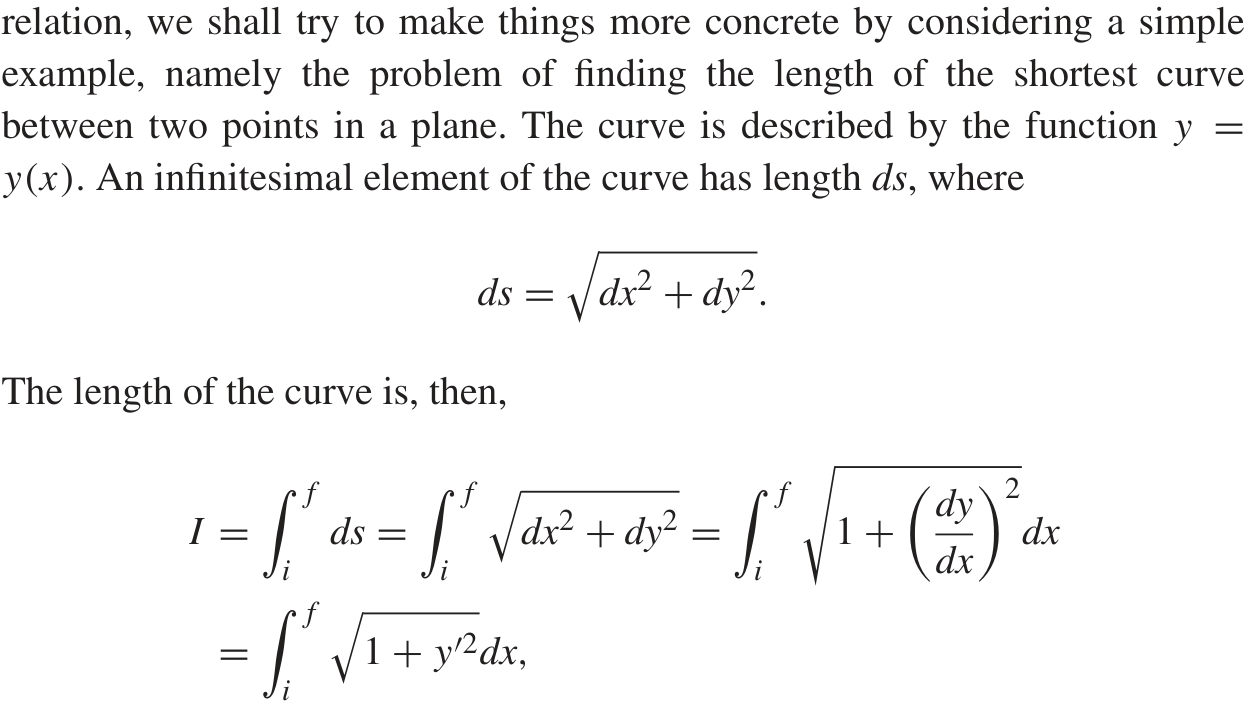
\includegraphics[width=0.55\linewidth]{../Figures/fig_2_1.png}
\caption{图 2.1 连接点 $i$ 与 $f$ 的曲线 $y = y(x)$}
\end{figure}

（为方便起见，我们把被积函数记为 $\Phi$。）现在假定你想求出对应于两终点之间最短路径长度的曲线。这意味着你要求一个函数 $y = y(x)$，使得积分 $I$ 为极小值。
积分可以写成下面的形式
$$
I = \int_i^f \Phi(y)\, dx,
\eqno\hbox{(2.1)}
$$
其中 $\Phi$ 是 $y$ 的函数。但 $y$ 本身是一个函数（它是 $x$ 的函数）。所以 $\Phi$ 是函数的函数。我们称它为泛函。
问题在于求出使泛函 $\Phi(y)$ 的积分为极小的函数 $y(x)$。对于我们正在讨论的情形，泛函显然是
$$
\Phi(y) = \sqrt{1 + y'^2}.
$$
可以想见，对于不同的问题，有不同的泛函。这里有一个不同的问题。确定一根无摩擦导线的形状 $z = z(x)$，使得受重力作用的一粒珠子从起点 $(x_i, z_i)$ 以最短时间滑落到终点 $(x_f, z_f)$。（这是一个著名的问题，牛顿在几个小时内就解决了它；它被称为最速降线问题。）在这个问题中，我们要使时间取极小值。一个物体从一点运动到另一点所需的时间等于距离除以速度。对沿导线滑落的质点，其速度可由能量守恒 $\frac{1}{2}mv^2 = mgh$ 求出，得
$$
v = \sqrt{2gh},
$$
其中 $h$ 是起点下方的距离。如果我们从 $z_i$ 起向下量取 $z$，则可写成 $v = \sqrt{2gz}$。于是沿曲线滑过距离 $ds$ 所需的时间为
$$
dt = \frac{ds}{\sqrt{2gz}} = \frac{\sqrt{dx^2 + dz^2}}{\sqrt{2gz}} = \sqrt{\frac{1 + z'^2}{2gz}}\, dx.
$$
这个问题中要求极小的量是
$$
I = \int_i^f \sqrt{\frac{1 + z'^2}{2gz}}\, dx,
$$
而泛函为
$$
\Phi(z, z') = \sqrt{\frac{1 + z'^2}{2gz}}.
\eqno\hbox{(2.2)}
$$
\begin{example}
测地线是球面上两点之间的最短距离。这是大圆的一段弧。最终我们将要求出大圆的方程，但在这里我们只求相应的泛函。

解 2.1 设半径为 $a$ 的球面上的一段路径微元为 $ds$，如图所示：
\begin{figure}[h]
\centering
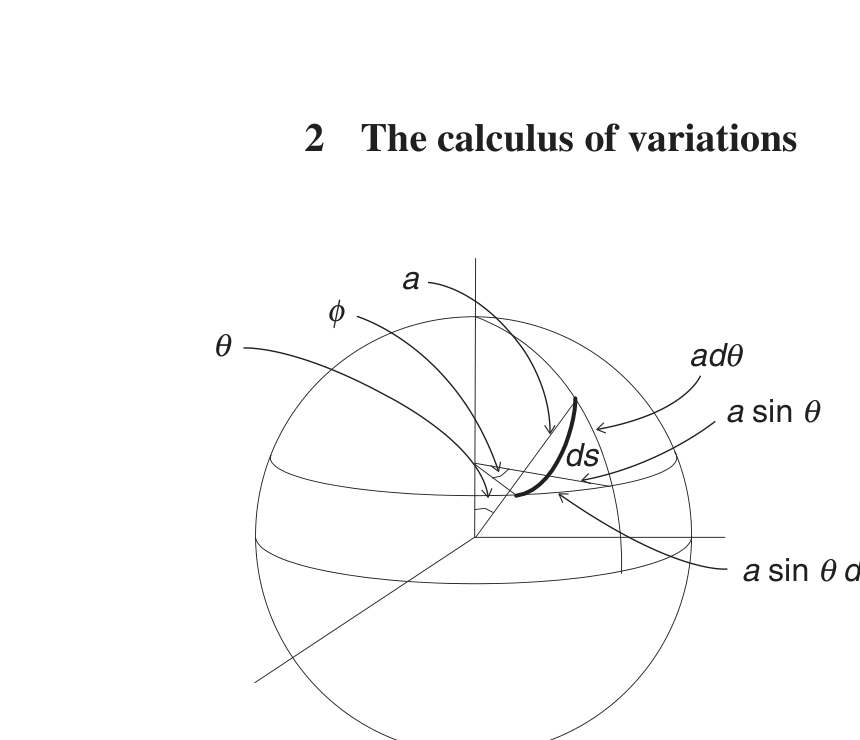
\includegraphics[width=0.55\linewidth]{../Figures/fig_2_2.png}
\caption{图 2.2 球面上的路径微元 $ds$}
\end{figure}
$$
ds^2 = a^2\,d\theta^2 + a^2 \sin^2\theta\, d\phi^2.
$$
因此，球面上一条曲线的长度为
$$
I = \int ds = \int a\,d\theta \sqrt{1 + \sin^2\theta\, \phi'^2},
$$
其中 $\phi' = d\phi/d\theta$。泛函为
$$
\Phi = \left(1 + \sin^2\theta\, \phi'^2\right)^{1/2}.
$$
\end{example}
在上述例子中得到的泛函具有变分法问题中泛函的典型形式。一般来说，我们将要用到的泛函依赖于两个函数，如 $y$ 与 $y'$，还依赖于参数 $x$，即
$$
\Phi = \Phi(x, y, y').
\eqno\hbox{(2.3)}
$$
注意 $y = y(x)$ 且 $y' = y'(x) = dy(x)/dx$。也就是说，$x$ 是自变量，而 $y$ 与 $y'$ 是 $x$ 的函数。（稍后我们将会把自变量取为时间 $t$ 来表述问题。）
到目前为止，我们所做的是描述最短距离、最速降线以及测地线等问题中泛函的求法。然而，我们还没有说明如何确定使积分取极小的那个函数。

现在让我们来推导积分取驻值的条件。我将以两点之间的最短路径为例，但推导是一般性的。设想在两点之间画一条直线。如你所知，这就是给出最短距离的路径。再设想在同样两点之间画出邻近的路径（即与最短路径相差无穷小的路径）。
\begin{figure}[h]
\centering
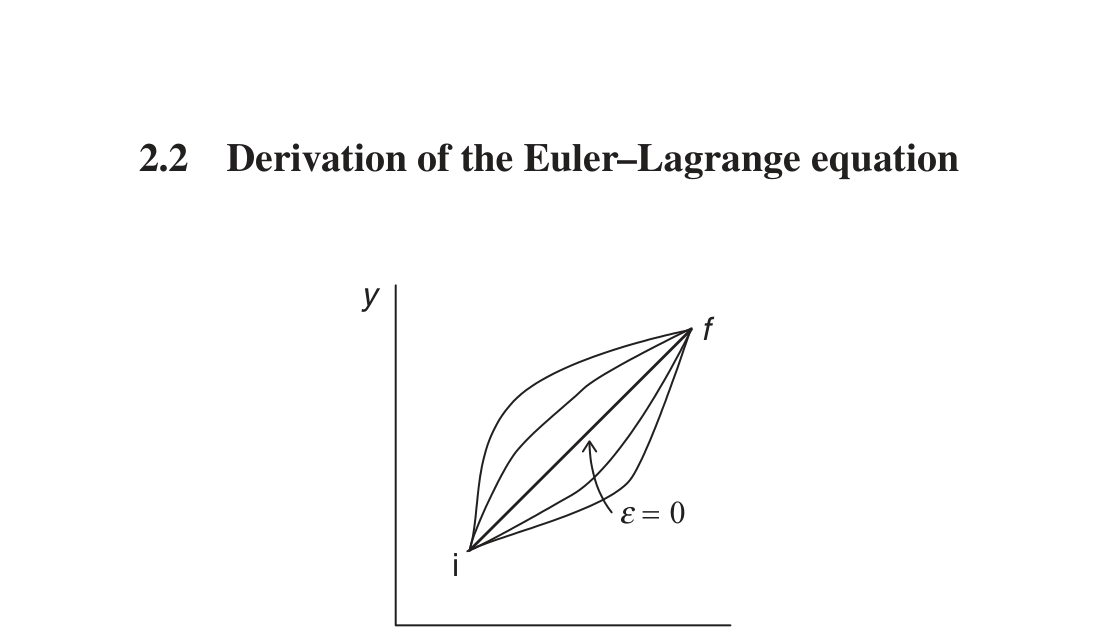
\includegraphics[width=0.55\linewidth]{../Figures/fig_2_3.png}
\caption{图 2.3 曲线族 $Y = y(x) + \epsilon\eta(x)$。最短距离曲线由 $\epsilon = 0$ 表示。注意所有曲线都在端点处相交，因此 $\eta(x_i) = \eta(x_f) = 0$。}
\end{figure}
若 $y = y(x)$ 是最小路径的方程，则邻近路径之一的方程可表示为
$$
Y(x, \epsilon) = y(x) + \epsilon\eta(x),
\eqno\hbox{(2.4)}
$$
其中 $\epsilon$ 是一个小量，$\eta(x)$ 是 $x$ 的任意函数，但它满足一个重要条件，即 $\eta(x)$ 在端点处必须为零，因为在这些点上所有路径都相交。对于给定的函数 $\eta(x)$，$\epsilon$ 的不同取值将给出不同的路径，它们都属于同一曲线族。（选取不同的函数 $\eta(x)$ 将产生另一族曲线，其中每条曲线都由 $\epsilon$ 的值表征。）假定 $\eta(x)$ 已给定，路径 $Y(x)$ 既是 $x$ 的函数，也是 $\epsilon$ 的函数。这就是我们把 $Y$ 写成 $Y = Y(x, \epsilon)$ 的原因。这些曲线中任一条的长度当然都依赖于 $\epsilon$ 的值，并可表示为
$$
I(\epsilon) = \int_{x_i}^{x_f} \Phi(x, Y, Y')\, dx,
$$
其中 $\Phi$ 具有如下形式：
$$
\Phi = \sqrt{1 + Y'^2}.
$$
我们把 $I$ 写成只依赖于 $\epsilon$ 的函数，因为对 $x$ 的依赖已经通过积分消去了。

我们想要确定使积分 $I$ 取驻值的函数 $y(x)$。在普通微积分中，我们会令微分为零（$dI = 0$）。但现在我们要问的是：函数 $y(x)$ 中哪一个使 $I$ 取驻值，于是我们令变分为零（$\delta I = 0$）。这常常被称为"一阶变分"，因为 $\delta I$ 是按马克劳林展开定义的：
$$
I(\epsilon) = I(0) + \left.\frac{dI}{d\epsilon}\right|_{\epsilon=0} \epsilon + O(\epsilon^2).
$$
只保留 $\epsilon$ 的一次项，我们定义
$$
\delta I(\epsilon) = I(\epsilon) - I(0) = \left.\frac{dI}{d\epsilon}\right|_{\epsilon=0} \epsilon.
$$
因此，$\delta I = 0$ 等价于
$$
\left.\frac{dI}{d\epsilon}\right|_{\epsilon=0} = 0.
$$
把 $I$ 的积分表达式代入，给出
$$
\left.\frac{d}{d\epsilon}\int_{x_i}^{x_f} \Phi(x, Y, Y')\, dx\right|_{\epsilon=0} = 0.
\eqno\hbox{(2.5)}
$$
$Y$ 与 $Y'$ 都是 $\epsilon$ 的函数。在积分号下求导，我们有
$$
\int_{x_i}^{x_f}\left[\frac{\partial\Phi}{\partial Y}\frac{\partial Y}{\partial\epsilon}
+ \frac{\partial\Phi}{\partial Y'}\frac{\partial Y'}{\partial\epsilon}\right]_{\epsilon=0}\, dx = 0.
\eqno\hbox{(2.6)}
$$
第二项可以如下进行分部积分：
$$
\int_{x_i}^{x_f} \frac{\partial\Phi}{\partial Y'}\frac{\partial Y'}{\partial\epsilon}\, dx
= \int_{x_i}^{x_f} \frac{\partial\Phi}{\partial Y'}\frac{\partial}{\partial\epsilon}\frac{dY}{dx}\, dx
= \int_{x_i}^{x_f} \frac{\partial\Phi}{\partial Y'}\frac{\partial}{\partial x}\frac{\partial Y}{\partial\epsilon}\, dx
= \left.\frac{\partial\Phi}{\partial Y'}\frac{\partial Y}{\partial\epsilon}\right|_{x_i}^{x_f}
- \int_{x_i}^{x_f} \frac{\partial}{\partial x}\left(\frac{\partial\Phi}{\partial Y'}\right)\frac{\partial Y}{\partial\epsilon}\, dx.
$$
但 $Y = y(x) + \epsilon\eta(x)$，所以 $\partial Y/\partial\epsilon = \eta(x)$，且在端点处 $\eta(x) = 0$（因为曲线在那里相交）。因此
$$
\left.\frac{\partial\Phi}{\partial Y'}\frac{\partial Y}{\partial\epsilon}\right|_{x_i}^{x_f}
= \frac{\partial\Phi}{\partial Y'}\left[\eta(x_f) - \eta(x_i)\right] = 0.
$$
于是，式 (2.6) 成为
$$
\int_{x_i}^{x_f}\left[\frac{\partial\Phi}{\partial Y}
- \frac{d}{dx}\left(\frac{\partial\Phi}{\partial Y'}\right)\right]
\left.\frac{\partial Y}{\partial\epsilon}\right|_{\epsilon=0}\, dx = 0.
\eqno\hbox{(2.7)}
$$
被积函数是两个函数的乘积。由于 $\partial Y/\partial\epsilon = \eta(x)$，式 (2.7) 具有如下形式：
$$
\int_a^b f(x)\eta(x)\, dx = 0,
\eqno\hbox{(2.8)}
$$
其中
$$
f(x) = \frac{\partial\Phi}{\partial Y} - \frac{d}{dx}\left(\frac{\partial\Phi}{\partial Y'}\right).
$$
函数 $\eta(x)$ 是任意的（端点处除外），所以式 (2.8) 成立当且仅当对所有 $x$ 的值都有 $f(x) = 0$。你可能会认为，要求所有 $x$ 都满足 $f(x) = 0$ 过于苛刻，但很容易说明事实并非如此。你可以这样理解：假定 $\eta(x)$ 除在 $x_i$ 与 $x_f$ 之间的某个点（比如 $x = x$）外处处为零。然后考虑积分
$$
\int_{x_f = x + \varepsilon}^{x_i = x - \varepsilon} f(x)\eta(x)\, dx = 0,
$$
其中 $\varepsilon$ 是一个很小的量。由于积分处处为零，它在上述积分区间内也为零。此外，$f(x)$ 在这个小区间上基本恒定。把它记为 $f(x)$，并移到积分号外：
$$
f(x)\int_{x_f = x + \varepsilon}^{x_i = x - \varepsilon} \eta(x)\, dx = 0.
$$
积分不为零，所以 $f(x)$ 必为零。但点 $x = x$ 可以位于 $x_i$ 到 $x_f$ 之间的任何地方，因此沿路径所有点处 $f(x)$ 均为零。
另一种论证 $\int_a^b f(x)\eta(x)\, dx = 0$ 蕴含 $f(x) = 0$ 的方法是：假定 $f(x)$ 不为零，并利用 $\eta(x)$ 的任意性。例如，我们可以要求在 $f(x)$ 为负的所有地方 $\eta(x)$ 取负值，在 $f(x)$ 为正的所有地方 $\eta(x)$ 取正值。但这样一来乘积 $f(x)\eta(x)$ 将处处为正，条件 (2.8) 便无法满足。于是我们再次得出结论：式 (2.8) 成立当且仅当 $f(x) = 0$。因此，式 (2.7) 化简为
$$
\left[\frac{\partial\Phi}{\partial Y}
- \frac{d}{dx}\left(\frac{\partial\Phi}{\partial Y'}\right)\right]_{\epsilon=0} = 0,
$$
这等价于要求
$$
\frac{\partial\Phi}{\partial y} - \frac{d}{dx}\left(\frac{\partial\Phi}{\partial y'}\right) = 0.
\eqno\hbox{(2.9)}
$$
这被称为欧拉-拉格朗日方程。\footnote{你在第一章（式 (1.16)）中已经遇到过欧拉-拉格朗日方程的一种变体。}它给出了 $y = y(x)$ 为使积分
$$
\int_{x_i}^{x_f} \Phi(x, y, y')\, dx
$$
取极小值的路径所必须满足的条件。例如，在求平面内两点之间最短距离的方程时，泛函为
$$
\Phi(x, y, y') = \sqrt{1 + y'^2}.
$$
把它代入欧拉-拉格朗日方程，我们得到
$$
-\frac{d}{dx}\left[\frac{\partial}{\partial y'}\left(1 + y'^2\right)^{1/2}\right] = 0,
$$
经过一些代数运算后，这给出
$$
y = mx + b,
$$
其中 $m$ 和 $b$ 为常数。但 $y = mx + b$ 正是直线的方程！

\begin{exercise}
证明泛函 $\Phi = \sqrt{1 + y'^2}$ 导出 $y = mx + b$。
\end{exercise}

\begin{exercise}
利用极坐标求平面上两点之间最短距离的方程。答案：$r\cos(\theta + \alpha) = C$，其中 $\alpha$ 与 $C$ 为常数。
\end{exercise}

\begin{exercise}
确定并识别使 $\int_{x_1}^{x_2} \left[x(1 + y'^2)\right]^{1/2}dx$ 取驻值的曲线 $y = y(x)$。答案：一条抛物线。
\end{exercise}

\begin{exercise}
确定并识别使 $\int_{x_1}^{x_2} \dfrac{ds}{y}$ 取驻值的曲线 $y = y(x)$。答案：一个圆。
\end{exercise}

\subsection*{2.2.1  变分 $\delta$ 与微分 $d$ 之间的差别}

变分 $\delta$ 与微分 $d$ 之间的差别不仅仅是记号上的。当作用于某个变量时，$\delta$ 表示虚位移，我们通常把它理解为在时间冻结的情况下坐标的变化。更一般地说，它是某个变量的一种虚的无穷小变化，即在保持自变量不变的条件下、以任意但在运动学上允许的方式所进行的变化。相比之下，我们把 $d$ 理解为某个变量在一段有限时间内发生的实际变化。
当作用于某个函数时，由拉格朗日引入的符号 $\delta$ 表示该函数的变分，而 $d$ 表示该函数的微分。作为一个简单例子，考虑函数 $F(x, \dot{x}, t)$，它是一个依赖于位置、速度和时间的函数。但位置和速度都依赖于时间。也就是说，时间是自变量，我们可以写成
$$
F = F(x(t), \dot{x}(t), t).
$$
按照微积分的法则，$F$ 的微分为
$$
dF = \frac{\partial F}{\partial x}\, dx + \frac{\partial F}{\partial \dot{x}}\, d\dot{x} + \frac{\partial F}{\partial t}\, dt.
$$
另一方面，$F$ 的变分为
$$
\delta F = \frac{\partial F}{\partial x}\, \delta x + \frac{\partial F}{\partial \dot{x}}\, \delta\dot{x}.
$$
微分与变分之间最显著的区别在于：微分使我们到达同一函数的不同点，而
\begin{figure}[h]
\centering
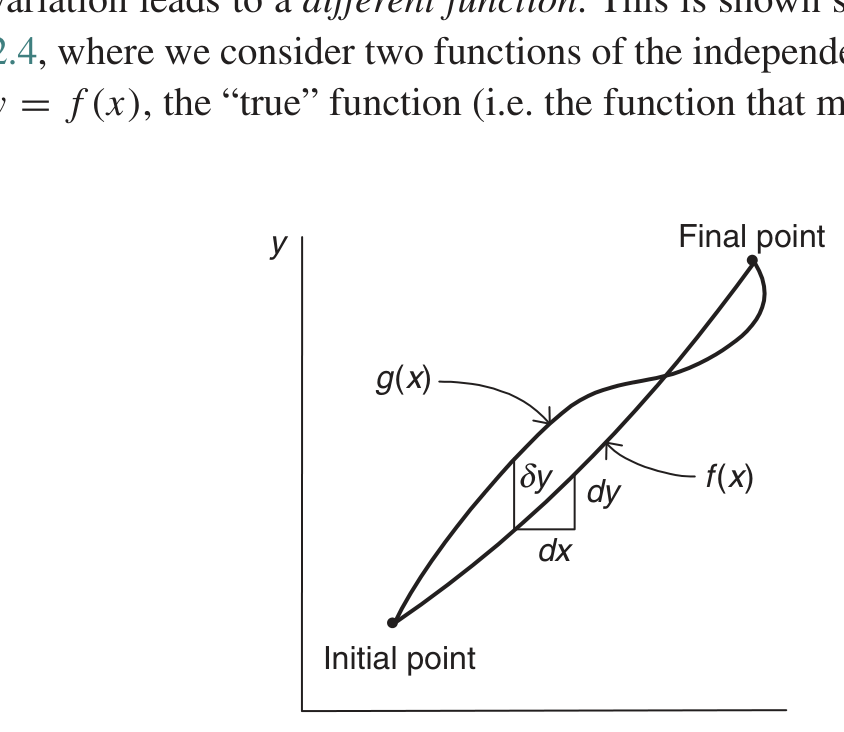
\includegraphics[width=0.55\linewidth]{../Figures/fig_2_4.png}
\caption{图 2.4 说明变分 $\delta$ 与微分 $d$ 之间差别的示意图}
\end{figure}
其中 $y = f(x)$ 是"真实"函数（即使定积分取极小的函数），而 $y = g(x) = f(x) + \epsilon\eta(x)$ 是具有相同端点的邻近函数，即"已变分"函数。变分 $\delta y$ 由下式给出：
$$
\delta y = g(x) - f(x).
$$
也就是说，$\delta y$ 给出真实函数与已变分函数在同一 $x$ 值处的差。另一方面，若 $y = f(x)$，则 $dy$ 是 $f(x)$ 由于 $x$ 的变化而产生的变化，即
$$
dy = f(x + dx) - f(x).
$$
当应用于定积分时，$\delta$ 与 $d$ 的差别变得尤为重要，因为两种变化常常同时起作用。

在欧拉-拉格朗日方程的推导中，我们使用 $\epsilon$ 作为参数，用来表示我们是在"真实"路径上（此时 $\epsilon = 0$）还是在某条已变分路径上（$\epsilon \neq 0$）。显然，给出路径长度的积分 $I$ 依赖于 $\epsilon$。这就是我们写成 $I = I(\epsilon)$ 的原因。下一步我们是求 $I$ 对 $\epsilon$ 的导数并令其为零。（$\epsilon$ 的不同取值把我们带到不同的曲线，即不同的函数 $y = y(x)$。）
我们也可以用变分来表示我们的问题，例如
$$
\delta y = \eta(x)\, d\epsilon,
$$
以及
$$
\delta y' = \eta'(x)\, d\epsilon.
$$
这些关系与表达式 $Y(x) = y(x) + \epsilon\eta(x)$ 一致。如果我们记得 $Y(x)$ 表示一族曲线 $y(x, \epsilon)$，那么把 $Y(x)$ 换成 $y(x, \epsilon)$，我们有
$$
\delta y = \delta\left[y(x, \epsilon)\right] = \left.\frac{dy(x, \epsilon)}{d\epsilon}\right|_{\epsilon=0}\delta\epsilon
= \left.\frac{d}{d\epsilon}\left(y(x) + \epsilon\eta(x)\right)\right|_{\epsilon=0}\delta\epsilon
= \eta(x)\,\delta\epsilon.
$$
由于 $I = I(y, y', x)$，我们有
$$
\delta I = \frac{\partial I}{\partial y}\, \delta y + \frac{\partial I}{\partial y'}\, \delta y'.
$$
（注意 $x$ 是冻结的。）但
$$
\delta I = \delta\int_{x_1}^{x_2} \Phi(y, y', x)\, dx
= \int_{x_1}^{x_2} \delta\Phi\, dx
= \int_{x_1}^{x_2}\left[\frac{\partial\Phi}{\partial y}\, \delta y
+ \frac{\partial\Phi}{\partial y'}\, \delta y'\right] dx
= \int_{x_1}^{x_2}\left[\frac{\partial\Phi}{\partial y}\, \eta(x)\, d\epsilon
+ \frac{\partial\Phi}{\partial y'}\, \eta'(x)\, d\epsilon\right] dx.
$$
因此，我们可以用两种方式中的任何一种来表达对 $I$ 的条件，即令
$$
\left.\frac{dI}{d\epsilon}\right|_{\epsilon=0} = 0
$$
正如我们在式 (2.7) 中所做的那样，或者断言变分 $\delta I$ 为零。这两种说法是等价的。
最后再就记号说几句。"泛函导数" $\Phi = \Phi(y, y', x)$ 的定义为
$$
\frac{\delta\Phi}{\delta y} = \frac{\partial\Phi}{\partial y}
- \frac{d}{dx}\left(\frac{\partial\Phi}{\partial y'}\right).
\eqno\hbox{(2.10)}
$$
它有时被称为"变分导数"。

\begin{exercise}
证明 $\delta$ 与 $d$ 对易。
\end{exercise}

\begin{exercise}
已知
$$
\delta\Phi = \frac{\partial\Phi}{\partial y}\, \delta y + \frac{\partial\Phi}{\partial y'}\, \delta y',
$$
证明 $\delta I = 0$ 与 $\left.\dfrac{dI}{d\epsilon}\right|_{\epsilon=0} = 0$ 表示同一件事。
\end{exercise}

\subsection*{2.2.2  欧拉-拉格朗日方程的等价形式}

我们把欧拉-拉格朗日方程推导成如下形式：
$$
\frac{\partial\Phi}{\partial y} - \frac{d}{dx}\left(\frac{\partial\Phi}{\partial y'}\right) = 0.
$$
这个表达式有两种变体。其中一种对 $\Phi$ 不依赖于 $y$ 的问题很有用，另一种对 $\Phi$ 不依赖于 $x$ 的问题很有用。
若 $\Phi$ 不依赖于 $y$，则欧拉-拉格朗日方程化简为
$$
\frac{d}{dx}\left(\frac{\partial\Phi}{\partial y'}\right) = 0,
$$
由此我们得出结论：
$$
\frac{\partial\Phi}{\partial y'} = \text{常数}.
$$
（这就是我们求解"平面内最短距离"问题时的情形。）
接下来假定 $\Phi$ 不依赖于 $x$。那么，由于 $\Phi = \Phi(y, y')$，$\Phi$ 对 $x$ 的偏导数为零，而 $\Phi$ 对 $x$ 的全导数将为
$$
\frac{d\Phi}{dx} = \frac{\partial\Phi}{\partial y}\frac{dy}{dx}
+ \frac{\partial\Phi}{\partial y'}\frac{dy'}{dx}.
$$
但 $\dfrac{dy'}{dx} = \dfrac{d}{dx}\left(\dfrac{dy}{dx}\right) = y''$，所以
$$
\frac{d\Phi}{dx} = \frac{\partial\Phi}{\partial y}\frac{dy}{dx}
+ y''\frac{\partial\Phi}{\partial y'} = y'\frac{\partial\Phi}{\partial y}
+ y''\frac{\partial\Phi}{\partial y'}.
\eqno\hbox{(2.11)}
$$
如果把欧拉-拉格朗日方程乘以 $y'$，我们得到
$$
y'\frac{\partial\Phi}{\partial y} - y'\frac{d}{dx}\left(\frac{\partial\Phi}{\partial y'}\right) = 0.
$$
在两边加上 $y''\,\partial\Phi/\partial y'$：
$$
y'\frac{\partial\Phi}{\partial y} - y'\frac{d}{dx}\left(\frac{\partial\Phi}{\partial y'}\right)
+ y''\frac{\partial\Phi}{\partial y'} = y''\frac{\partial\Phi}{\partial y'}.
$$
即
$$
y'\frac{\partial\Phi}{\partial y} + y''\frac{\partial\Phi}{\partial y'}
= y''\frac{\partial\Phi}{\partial y'} + y'\frac{d}{dx}\left(\frac{\partial\Phi}{\partial y'}\right).
$$
左端正是 $d\Phi/dx$（见式 (2.11)），而右端是
$$
\frac{d}{dx}\left(y'\frac{\partial\Phi}{\partial y'}\right),
$$
所以
$$
\frac{d\Phi}{dx} = \frac{d}{dx}\left(y'\frac{\partial\Phi}{\partial y'}\right),
$$
或
$$
\frac{d}{dx}\left(\Phi - y'\frac{\partial\Phi}{\partial y'}\right) = 0.
$$
因此，
$$
\Phi - y'\frac{\partial\Phi}{\partial y'} = \text{常数}.
\eqno\hbox{(2.12)}
$$

\begin{example}
最速降线问题：问题是确定导线的形状，使得导线上的珠子从某个起点以最短时间滑落到某个较低的终点。注意两个端点 $(x_1, z_1)$ 和 $(x_2, z_2)$ 是固定的。在 2.2 节中我们已经求出了泛函。现在我们求解曲线 $z = z(x)$。
解 2.2 泛函由式 (2.2) 给出：
$$
\Phi(z, z') = \sqrt{\frac{1 + z'^2}{2gz}}.
$$
注意 $\Phi$ 不依赖于 $x$。因此，
$$
\Phi - z'\frac{\partial\Phi}{\partial z'} = \text{常数}.
$$
因子 $2g$ 可以弃去。完成运算后，我们得到
$$
\sqrt{\frac{1 + z'^2}{z}} - \frac{z'^2}{\sqrt{z}\sqrt{1 + z'^2}}
= \text{常数} = 1/C.
\eqno\hbox{(2.13)}
$$
这可以表示为
$$
z(1 + z'^2) = C.
\eqno\hbox{(2.14)}
$$
细节留作练习。我们可以令
$$
z' = \cot\theta
$$
来得到这个微分方程的一个解。于是 $1 + z'^2 = 1/\sin^2\theta$，我们的微分方程可以写成
$$
z(1 + \cot^2\theta) = z/\sin^2\theta = C,
$$
或
$$
z = C\sin^2\theta.
$$
接下来注意
$$
\frac{dx}{d\theta} = \frac{dx}{dz}\frac{dz}{d\theta} = \frac{1}{z'}\frac{dz}{d\theta}
= \tan\theta\,\frac{dz}{d\theta}
= \tan\theta\,\frac{d}{d\theta}\left(C\sin^2\theta\right) = C(1 - \cos 2\theta).
$$
因此
$$
x = \int C(1 - \cos 2\theta)\, d\theta
= C\left(\theta - \frac{1}{2}\sin 2\theta\right).
$$
令 $C = 2A$ 且 $2\theta = \phi$，我们可把 $x$ 与 $z$ 写成如下参数方程：
$$
x = A(\phi - \sin\phi)
$$
$$
z = A(1 - \cos\phi).
$$
这些是摆线的参数方程。因此，若导线弯成摆线形，珠子就能以最短时间从 $(x_1, z_1)$ 滑落到 $(x_2, z_2)$。
\end{example}

\begin{exercise}
证明欧拉-拉格朗日方程的以下两种形式等价：
$$
\frac{\partial\Phi}{\partial y} - \frac{d}{dx}\left(\frac{\partial\Phi}{\partial y'}\right) = 0
$$
和
$$
\frac{\partial\Phi}{\partial x} - \frac{d}{dx}\left(\Phi - y'\frac{\partial\Phi}{\partial y'}\right) = 0,
$$
假设 $y' \neq 0$。
\end{exercise}

\begin{exercise}
由式 (2.13) 出发导出式 (2.14)。
\end{exercise}

\begin{exercise}
求珠子从点 $(-\pi, 2)$ 沿导线滑落到 $(0, 0)$（单位：米）所需的最短时间。答案：$\pi/\sqrt{g}$。
\end{exercise}

\section*{2.3  推广到多个因变量}

我们一直在考虑泛函具有 $\Phi = \Phi(x, y, y')$ 形式的问题。在本节中，我们把结果推广到依赖于 $n$ 个因变量 $y_1, y_2, \ldots, y_n$ 及其导数 $y'_1, y'_2, \ldots, y'_n$ 的泛函。我们假定这些变量彼此独立。\footnote{本节是为了完整起见而包含的。其过程是对上一节 (2.2) 所述较简单情形的推广。你可以跳过本节而不影响内容的连贯性，但请注意，此处得到的某些结果将在 3.4 节中使用。}
现在系统的泛函为 $\Phi(y_1, y_2, \ldots, y_n, y'_1, y'_2, \ldots, y'_n, x)$。我们将证明，这将导致 $n$ 个具有如下形式的欧拉-拉格朗日方程：
$$
\frac{\partial\Phi}{\partial y_i} - \frac{d}{dx}\left(\frac{\partial\Phi}{\partial y'_i}\right) = 0,
\qquad i = 1, \ldots, n.
$$
推导过程与前节所述类似，但更为一般。
回想我们的目的是确定使定积分
$$
I = \int_{x_i}^{x_f} \Phi(y_1, \ldots, y_n, y'_1, \ldots, y'_n, x)\, dx
$$
取极小（或极大）值的函数 $y_1(x), y_2(x), \ldots$。也就是说，我们要求出使
$$
\delta I = 0
$$
的函数 $y_i(x)$。
如前所述，端点之间存在无穷多条路径。与最小路径（即真实路径）相差无穷小的路径可以描述为
$$
Y_i(x) = y_i(x) + \epsilon\eta_i(x).
$$
积分 $I$ 依赖于所选路径，所以它可以被看作 $\epsilon$ 的函数。
$I$ 的变分为
$$
\delta I = \delta\int_{x_i}^{x_f} \Phi\, dx
= \int_{x_i}^{x_f} \delta\Phi\, dx
= \int_{x_i}^{x_f}\left[\frac{\partial\Phi}{\partial Y_i}\delta Y_i
+ \frac{\partial\Phi}{\partial Y'_i}\delta Y'_i\right] dx.
$$
把 $Y_i$ 与 $Y'_i$ 看作 $\epsilon$ 的函数，我们写成
$$
\delta I = \left.\frac{\partial I}{\partial\epsilon}\right|_{\epsilon=0} d\epsilon
= \int_{x_i}^{x_f}\left[\frac{\partial\Phi}{\partial Y_i}\frac{\partial Y_i}{\partial\epsilon}
+ \frac{\partial\Phi}{\partial Y'_i}\frac{\partial Y'_i}{\partial\epsilon}\right]_{\epsilon=0} d\epsilon.
$$
第二项可以分部积分。（注意这里的数学过程与由式 (2.6) 到式 (2.7) 的过程几乎完全相同。）我们有
$$
\int_{x_i}^{x_f} \frac{\partial\Phi}{\partial Y'_i}\frac{\partial Y'_i}{\partial\epsilon}\, d\epsilon\, dx
= \int_{x_i}^{x_f} \frac{\partial\Phi}{\partial Y'_i}\frac{\partial^2 Y_i}{\partial\epsilon\,\partial x}\, dx\, d\epsilon
= \int_{x_i}^{x_f} \frac{\partial\Phi}{\partial Y'_i}\frac{\partial}{\partial\epsilon}\frac{\partial Y_i}{\partial x}\, dx\, d\epsilon
$$
$$
= \left.\frac{\partial\Phi}{\partial Y'_i}\frac{\partial Y_i}{\partial\epsilon}\right|_{x_1}^{x_2}
- \int_{x_i}^{x_f}\frac{\partial Y_i}{\partial\epsilon}\frac{\partial}{\partial x}\left(\frac{\partial\Phi}{\partial Y'_i}\right) dx\, d\epsilon
= - \int_{x_i}^{x_f}\frac{\partial Y_i}{\partial\epsilon}\frac{\partial}{\partial x}\left(\frac{\partial\Phi}{\partial Y'_i}\right) dx\, d\epsilon,
$$
其中我们用到了事实 $\left.\dfrac{\partial Y_i}{\partial\epsilon}\right|_{x_1}^{x_2} = 0$，因为所有曲线都通过端点。
因此，
$$
\delta I = \int_{x_i}^{x_f}\left[\frac{\partial\Phi}{\partial Y_i}\frac{\partial Y_i}{\partial\epsilon}
- \frac{\partial Y_i}{\partial\epsilon}\frac{\partial}{\partial x}\left(\frac{\partial\Phi}{\partial Y'_i}\right)\right] d\epsilon\, dx
$$
$$
= \int_{x_i}^{x_f}\left[\frac{\partial\Phi}{\partial Y_i}
- \frac{d}{dx}\left(\frac{\partial\Phi}{\partial Y'_i}\right)\right]\frac{\partial Y_i}{\partial\epsilon}\, d\epsilon\, dx
= \int_{x_i}^{x_f}\left[\frac{\partial\Phi}{\partial Y_i}
- \frac{d}{dx}\left(\frac{\partial\Phi}{\partial Y'_i}\right)\right]\delta Y_i\, dx.
$$
当 $\epsilon = 0$ 时，$\delta I = 0$，因为 $I$ 是沿路径 $y_i = y_i(x)$ 取极小的。所以
$$
\left[\delta I\right]_{\epsilon=0} = 0 = \int_{x_i}^{x_f}\left[\frac{\partial\Phi}{\partial y_i}
- \frac{d}{dx}\left(\frac{\partial\Phi}{\partial y'_i}\right)\right]\delta y_i\, dx.
\eqno\hbox{(2.15)}
$$
由于各 $\delta y_i$ 相互独立，这个表达式为零的唯一方式是括号中的所有项都为零。因此，
$$
\frac{\partial\Phi}{\partial y_i} - \frac{d}{dx}\left(\frac{\partial\Phi}{\partial y'_i}\right) = 0,
\qquad i = 1, \ldots, n,
\eqno\hbox{(2.16)}
$$
正如所预期的那样。

\section*{2.4  约束}

变分法中的许多问题都涉及约束，或者如它们有时被称呼的那样——"附加条件"。例如，一个质点可能被约束在 $z = 0$ 平面内，或约束为沿某条特定曲线运动。

\subsection*{2.4.1  完整约束}

让我们从考虑完整约束开始。回想 1.4 节，完整约束是因变量之间的这样一种关系：它可以表示为一个等于零的函数。在存在约束的情况下，因变量彼此并不独立，它们由附加条件联系在一起。例如，让我们考虑一个问题，它由 $\Phi = \Phi(y_1, \ldots, y_n; y'_1, \ldots, y'_n; x)$ 描述，其中 $n$ 个因变量受 $m$ 个如下形式的约束联系：
$$
f_1(y_1, y_2, \ldots, y_n, x) = 0,
$$
$$
\vdots
$$
$$
f_m(y_1, y_2, \ldots, y_n, x) = 0.
$$
每个约束使自由度的数目减少一个。若有 $n$ 个因坐标和 $m$ 个约束，我们可以利用这些约束把自由度的数目减少到 $n - m$，然后应用 $n - m$ 个欧拉-拉格朗日方程来求解问题。这在概念上很简单，但在实践中可能相当复杂。更好的方法是保留全部 $n$ 个变量，使用拉格朗日乘子法。我们现在就来考虑这种方法（常被称为拉格朗日 $\lambda$ 法）。我们首先对约束方程取变分，即：
$$
\delta f_1 = \frac{\partial f_1}{\partial y_1}\delta y_1 + \frac{\partial f_1}{\partial y_2}\delta y_2
+ \cdots + \frac{\partial f_1}{\partial y_n}\delta y_n = 0,
$$
$$
\vdots
$$
$$
\delta f_m = \frac{\partial f_m}{\partial y_1}\delta y_1 + \frac{\partial f_m}{\partial y_2}\delta y_2
+ \cdots + \frac{\partial f_m}{\partial y_n}\delta y_n = 0.
\eqno\hbox{(2.17)}
$$
接下来，我们把每个这样的关系式乘以一个"待定乘子" $\lambda_i$ 并把它们相加，得到
$$
\lambda_1\delta f_1 + \lambda_2\delta f_2 + \cdots + \lambda_m\delta f_m = 0.
\eqno\hbox{(2.18)}
$$
这个和为零，因为每个 $\delta f$ 都为零。
我们还知道，泛函 $\Phi$ 的变分在驻点处消失。也就是说，
$$
\delta\Phi = \frac{\partial\Phi}{\partial y_1}\delta y_1 + \frac{\partial\Phi}{\partial y_2}\delta y_2
+ \cdots + \frac{\partial\Phi}{\partial y_n}\delta y_n = 0.
\eqno\hbox{(2.19)}
$$
式 (2.18) 与式 (2.19) 之和也必为零，所以我们有
$$
0 = \frac{\partial\Phi}{\partial y_1}\delta y_1 + \frac{\partial\Phi}{\partial y_2}\delta y_2
+ \cdots + \frac{\partial\Phi}{\partial y_n}\delta y_n
$$
$$
+ \lambda_1\left(\frac{\partial f_1}{\partial y_1}\delta y_1 + \frac{\partial f_1}{\partial y_2}\delta y_2
+ \cdots + \frac{\partial f_1}{\partial y_n}\delta y_n\right)
$$
$$
+ \cdots + \lambda_m\left(\frac{\partial f_m}{\partial y_1}\delta y_1 + \frac{\partial f_m}{\partial y_2}\delta y_2
+ \cdots + \frac{\partial f_m}{\partial y_n}\delta y_n\right).
\eqno\hbox{(2.20)}
$$
这个表达式很复杂，所以为了说明其过程，我将假定只有一个约束。（推广到 $m$ 个约束的情况留作习题。）如果只有一个约束，式 (2.18) 可以写成
$$
\lambda\,\delta f = \lambda\left(\frac{\partial f}{\partial y_1}\delta y_1 + \frac{\partial f}{\partial y_2}\delta y_2
+ \cdots + \frac{\partial f}{\partial y_n}\delta y_n\right) = 0,
\eqno\hbox{(2.21)}
$$
而式 (2.20) 化简为
$$
\frac{\partial\Phi}{\partial y_1}\delta y_1 + \frac{\partial\Phi}{\partial y_2}\delta y_2
+ \cdots + \frac{\partial\Phi}{\partial y_n}\delta y_n
+ \lambda\left(\frac{\partial f}{\partial y_1}\delta y_1 + \frac{\partial f}{\partial y_2}\delta y_2
+ \cdots + \frac{\partial f}{\partial y_n}\delta y_n\right) = 0.
$$
重新整理得到
$$
\sum_{i=1}^{n}\left(\frac{\partial\Phi}{\partial y_i} + \lambda\frac{\partial f}{\partial y_i}\right)\delta y_i = 0.
$$
由于 $\lambda$ 是我们任意引入的，我们可以自由地给它任何我们想要的值。让我们选取 $\lambda$，使求和中的第 $n$ 项为零。也就是说，$\lambda$ 的值由要求
$$
\frac{\partial\Phi}{\partial y_n} + \lambda\frac{\partial f}{\partial y_n} = 0
\eqno\hbox{(2.22)}
$$
来确定。于是求和中的第 $n$ 项被消去，留下
$$
\sum_{i=1}^{n-1}\left(\frac{\partial\Phi}{\partial y_i} + \lambda\frac{\partial f}{\partial y_i}\right)\delta y_i = 0.
$$
现在所有的 $\delta y$ 都相互独立，而求和为零当且仅当每个变分 $\delta y_i$（$i = 1, \ldots, n - 1$）的系数为零。也就是说，
$$
\frac{\partial\Phi}{\partial y_i} + \lambda\frac{\partial f}{\partial y_i} = 0,
\qquad i = 1, 2, \ldots, n - 1.
\eqno\hbox{(2.23)}
$$
注意我们没有消去任何变量。我们可以把式 (2.21)、(2.22) 和 (2.23) 相加，得到
$$
\delta\Phi + \lambda\,\delta f = 0.
$$
这可以写成
$$
\delta(\Phi + \lambda f) = 0,
\eqno\hbox{(2.24)}
$$
因为 $\delta(\lambda f) = f\,\delta\lambda + \lambda\,\delta f = \lambda\,\delta f$（由于 $f = 0$）。
式 (2.24) 表明：对于广义坐标的任意变分，$\Phi + \lambda f$ 的变分为零。这样，我们就重新表述了这个问题。最初我们有受约束 $f(y_1 \ldots y_n) = 0$ 限制的 $\delta\Phi = 0$，而现在我们有不带坐标约束的 $\delta(\Phi + \lambda f) = 0$。原来的问题有 $n-1$ 个自由度，而重新表述的问题把所有坐标都当作无约束的，并引入了另一个变量 $\lambda$，从而给出 $n+1$ 个自由度。进一步注意，$\delta(\Phi + \lambda f) = 0$ 给出 $n$ 个方程，而 $f = 0$ 是又一个方程。因此我们有 $n + 1$ 个方程对应 $n + 1$ 个未知量。

\begin{example}
作为前述方法一个非常简单的应用，考虑平面 $\Phi(x, y) = x + y$。$xy$ 平面中的一个圆向上投影到 $\Phi$ 平面上，如
\begin{figure}[h]
\centering
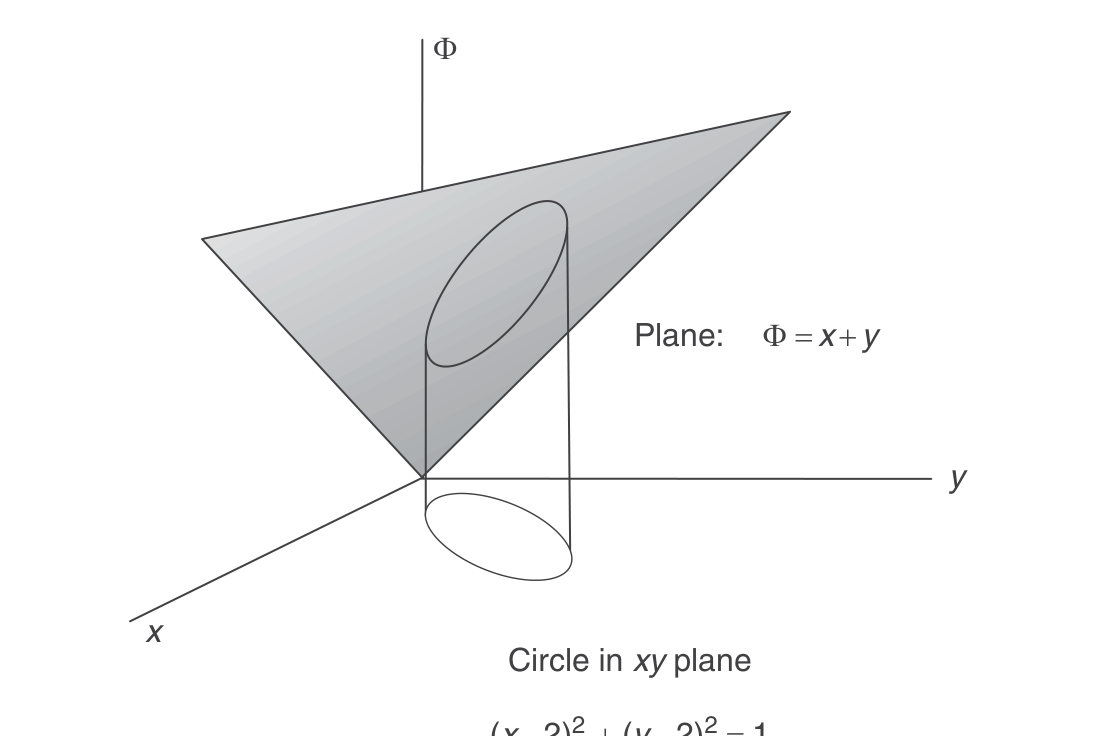
\includegraphics[width=0.55\linewidth]{../Figures/fig_2_5.png}
\caption{图 2.5 $xy$ 平面中的圆向上投影到阴影曲面上}
\end{figure}
图所示。在约束 $(x - 2)^2 + (y - 2)^2 = 1$ 下，求投影圆各点处 $\Phi$ 的极大值与极小值。
解 2.3 已知
$$
\Phi(x, y) = x + y,
$$
$$
f(x, y) = (x - 2)^2 + (y - 2)^2 - 1 = 0,
$$
条件
$$
\delta(\Phi + \lambda f) = 0,
$$
当代入欧拉-拉格朗日方程时，给出下面三个方程
$$
\frac{\partial}{\partial x}(\Phi + \lambda f) = 0 \quad\implies\quad 1 + \lambda\left(2(x - 2)\right) = 0,
$$
$$
\frac{\partial}{\partial y}(\Phi + \lambda f) = 0 \quad\implies\quad 1 + \lambda\left(2(y - 2)\right) = 0,
$$
$$
\frac{\partial}{\partial \lambda}(\Phi + \lambda f) = 0 \quad\implies\quad (x - 2)^2 + (y - 2)^2 - 1 = 0.
$$
第三个方程就是约束本身。第一和第二个方程可以解出 $\lambda$。令 $\lambda$ 的两个表达式相等，我们得到
$$
2x - 4 = 2y - 4
$$
由此得 $x = y$。把它代入第三个方程，我们得到
$$
2(x - 2)^2 = 1
$$
由此
$$
x = 2 \pm 1/\sqrt{2},
$$
因此极值点位于
$$
(1.29, 1.29) \quad\text{和}\quad (2.71, 2.71).
$$
\end{example}

\subsection*{2.4.2  非完整约束}

微分约束
假定约束不是变量之间的代数关系，而是一个微分关系。例如，"无滑动滚动"约束表示为线位移与角位移之间的如下关系：
$$
ds = r\,d\theta.
$$
除以 $dt$，你会注意到这是速度之间的关系，而不是坐标之间的关系。显然，如果你能对微分之间的关系进行积分，你就会得到一个完整约束，然后就可以像前面那样继续处理。如果约束真正是非完整的，也并非没有办法，因为对某些非完整约束，可以应用上面描述的拉格朗日 $\lambda$ 法。假定约束表示为如下形式：
$$
A_1\,\delta y_1 + A_2\,\delta y_2 + \cdots + A_n\,\delta y_n = 0.
$$
这里要指出两点。首先，式 (2.17) 中出现的偏导数被系数 $A_i$ 取代，它们是因变量的函数，但不是某个函数的导数。其次，我们不能消去变量，因为我们没有所需要的、能把一个变量用其他变量表示出来的那些方程。尽管如此，拉格朗日 $\lambda$ 法仍然可以应用。定义量 $\delta f$：
$$
\delta f = A_1\,\delta y_1 + A_2\,\delta y_2 + \cdots + A_n\,\delta y_n = 0.
$$
把 $\delta f$ 乘以 $\lambda$ 并加到泛函 $\Phi$ 的变分上：
$$
\delta\Phi + \lambda\,\delta f = 0.
$$
现在，再一次，你可以把所有 $\delta y_i$ 都当作独立的来处理。
如果附加条件是依赖于时间的（非定常的），其过程会稍微复杂一些，我们不予考虑。有兴趣的学生可以阅读 Lanczos 著作的 2.13 节\footnote{C. Lanczos, The Variational Principles of Mechanics, 4th ed., Dover, New York (1986).}以获得简要的讨论。

等周约束
有些约束以积分的形式表示。这样的约束被称为"等周条件"，因为这类问题中最著名的就是"狄多女王"问题，即求具有给定周长、围出最大面积的曲线。\footnote{传说中，狄多女王为逃避她的兄长而去了迦太基。她提出要购买土地，但该城的统治者傲慢地告诉她，她只能拥有用一张牛皮所能围出的那么多土地。狄多把她能找到的最大一头牛的牛皮切成了尽可能细的条。问题是：在给定皮条长度的条件下，证明圆形围出的面积最大。}一般说来，约束以具有给定定值的定积分给出，即
$$
\int_{x_1}^{x_2} f(x, y, y')\, dx = C,
\eqno\hbox{(2.25)}
$$
其中 $C$ 为已知。这类问题可以用拉格朗日 $\lambda$ 法求解。假定要求极大值的积分为
$$
I = \int_{x_1}^{x_2} \Phi(x, y, y')\, dx.
\eqno\hbox{(2.26)}
$$
为简单起见，让我们考虑只受一个约束的系统。（推广到多个具有式 (2.25) 形式的条件的情形是直截了当的。）条件 (2.25) 的变分为
$$
\delta\int_{x_1}^{x_2} f(x, y, y')\, dx
= \int_{x_1}^{x_2}\left[\frac{\partial f}{\partial y}\delta y
+ \frac{\partial f}{\partial y'}\delta y'\right] dx = 0.
\eqno\hbox{(2.27)}
$$
把式 (2.27) 乘以待定常数 $\lambda$ 并加到 $\delta I$ 上，得到
$$
\delta\int_{x_1}^{x_2} (\Phi + \lambda f)\, dx = 0.
$$
因此，拉格朗日 $\lambda$ 法意味着积分
$$
\int_{x_1}^{x_2} (\Phi + \lambda f)\, dx
$$
是驻值，因而被积函数满足欧拉-拉格朗日方程。注意约束与泛函的积分具有相同的积分限。

\begin{example}
确定长度为 $L$ 的曲线围出最大面积时的形状。
解 2.4 回顾微积分可知，曲线 $C$ 所围的面积由下式给出：
$$
\text{面积} = A = \frac{1}{2}\oint(x\, dy - y\, dx).
$$
把 $x$ 和 $y$ 用参数表示成 $x(t)$ 和 $y(t)$，我们写成
$$
A = \frac{1}{2}\int\left(x\frac{dy}{dt} - y\frac{dx}{dt}\right)dt
= \frac{1}{2}\int (xy' - yx')\, dt.
$$
（这里 $t$ 只是一个参数——它不是时间。）曲线长度为 $L$ 的约束是
$$
f = \int \sqrt{x'^2 + y'^2}\, dt - L = 0.
$$
注意 $\Phi = \Phi(x, y, x', y', t)$，其中 $t$ 为自变量。由于 $\Phi + \lambda f$ 是驻值，它满足如下的欧拉-拉格朗日方程：
$$
\frac{\partial(\Phi + \lambda f)}{\partial x}
- \frac{d}{dt}\left(\frac{\partial(\Phi + \lambda f)}{\partial x'}\right) = 0,
$$
$$
\frac{\partial(\Phi + \lambda f)}{\partial y}
- \frac{d}{dt}\left(\frac{\partial(\Phi + \lambda f)}{\partial y'}\right) = 0,
$$
得出
$$
\frac{1}{2}y' - \frac{d}{dt}\left(-\frac{1}{2}y + \frac{\lambda x'}{\sqrt{x'^2 + y'^2}}\right) = 0,
$$
$$
-\frac{1}{2}x' - \frac{d}{dt}\left(\frac{1}{2}x + \frac{\lambda y'}{\sqrt{x'^2 + y'^2}}\right) = 0.
$$
积分一次，我们得到
$$
\frac{1}{2}y + \frac{1}{2}y - \frac{\lambda x'}{\sqrt{x'^2 + y'^2}} = C_2,
$$
$$
-\frac{1}{2}x - \frac{1}{2}x - \frac{\lambda y'}{\sqrt{x'^2 + y'^2}} = -C_1,
$$
其中 $C_1$ 与 $C_2$ 是积分常数。重新整理，我们写成
$$
y - C_2 = \frac{\lambda x'}{\sqrt{x'^2 + y'^2}},
$$
$$
x - C_1 = \frac{\lambda y'}{\sqrt{x'^2 + y'^2}}.
$$
因此，对两式平方并相加，得到
$$
(x - C_1)^2 + (y - C_2)^2
= \frac{\lambda^2}{x'^2 + y'^2}(x'^2 + y'^2) = \lambda^2,
$$
这是一个圆心在 $(C_1, C_2)$、半径为 $\lambda$ 的圆的方程。
\end{example}

\section*{2.5  习题}

2.1 把拉格朗日 $\lambda$ 法推广到具有 $n$ 个坐标和 $m$ 个约束（$m < n$）的系统，并证明
$$
\delta(\Phi + \lambda_1 f_1 + \cdots + \lambda_m f_m) = 0,
$$
其中 $\lambda$ 由
$$
\frac{\partial\Phi}{\partial q_i} + \lambda_1\frac{\partial f_1}{\partial q_i}
+ \cdots + \lambda_m\frac{\partial f_m}{\partial q_i} = 0,
\qquad i = n - m + 1, \ldots, n
$$
求出。

2.2 确定圆锥面上两点之间最短距离所对应的曲线方程。设 $r^2 = x^2 + y^2$ 且 $z = r\cot\alpha$。

2.3 确定柱面（$r = 1 + \cos\theta$）上两点之间最短曲线所对应的方程。

2.4 考虑一个高度给定的旋转体。若该旋转体关于其轴线的转动惯量最小，确定它的形状。

2.5 考虑端点可变的变分问题。（a）设
$$
I = \int_a^b \Phi(x, y, y')\, dx,
$$
其中 $y(b)$ 是任意的。证明
$$
\delta I = \left.\eta\,\frac{\partial\Phi}{\partial y'}\right|_a^b
+ \int_a^b\left(\frac{\partial\Phi}{\partial y}
- \frac{d}{dx}\frac{\partial\Phi}{\partial y'}\right)\eta\, dx,
$$
条件为
$$
\left.\frac{\partial\Phi}{\partial y'}\right|_{x=b} = 0.
$$
（b）假定在 $x = a$ 处 $y$ 固定，但另一个端点可以位于曲线 $g(x, y) = 0$ 上的任意位置。证明除了欧拉-拉格朗日条件之外，我们还有
$$
\left(\Phi - y'\frac{\partial\Phi}{\partial y'}\right)\frac{\partial g}{\partial y}
- \frac{\partial\Phi}{\partial y'}\frac{\partial g}{\partial x} = 0.
$$
\begin{figure}[h]
\centering
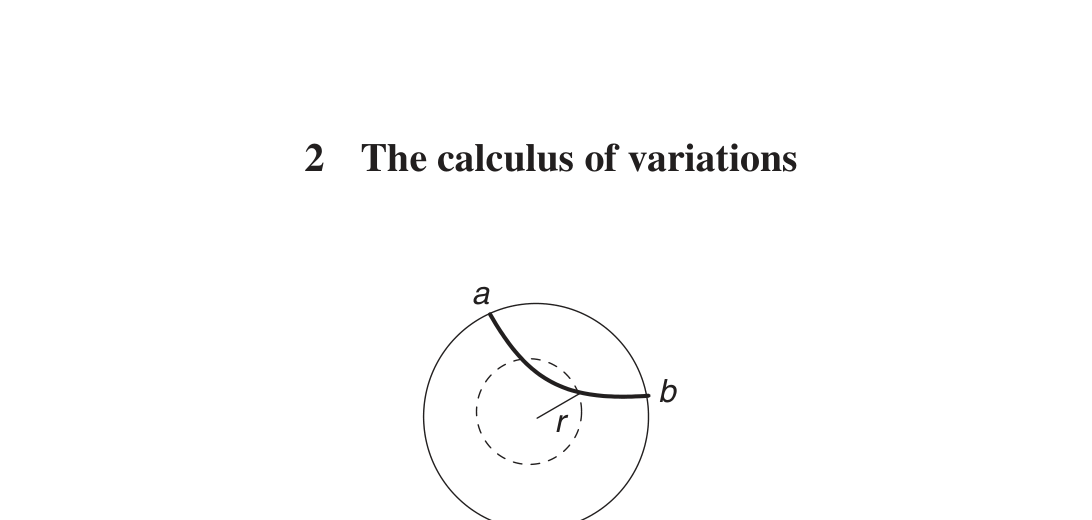
\includegraphics[width=0.55\linewidth]{../Figures/fig_2_6.png}
\caption{图 2.6 用于地球两点间快速穿行的无摩擦隧道}
\end{figure}

2.6 从点 $a$ 到点 $b$ 挖一条穿过地球的无摩擦隧道。从入口处丢下的物体将在重力作用下滑过隧道，并在另一端以零速度出来。地球内部某点的引力势为 $\phi = -Gm_s/r$，其中 $m_s$ 是半径为 $r$ 的球体所包围物质的体积。\footnote{见 P. W. Cooper, Through the Earth in forty minutes, Am. J. Phys., 34, 68 (1966) 以及 G. Venezian, Terrestrial brachistochrone, Am. J. Phys., 34, 701 (1966)。}（我们假定地球密度恒定。）利用极坐标，求出使时间 $dt$ 取极小的路径方程。

2.7 两个半径为 $a$ 的圆环相距 $2b$ 放置。（两圆环的圆心在同一条直线上，且圆环所在平面垂直于这条直线。）求在两圆环之间形成的皂膜的形状，注意皂膜将具有最小的表面积。

2.8 质量为 $m$ 的质点在二维力场
$$
\mathbf{F} = -\frac{GMm}{r^2}\hat{r}
$$
中运动。使质点从一点落到另一点所需时间最短的曲线是微分方程
$$
\frac{dr}{d\theta} = f(r)
$$
的解。求 $f(r)$。

2.9 考虑函数
$$
f(x, y, z) = x^2 + 2y^2 + 3z^2 + 2xy + 2xz,
$$
在条件
$$
x^2 + y^2 + z^2 = 1
$$
下，$f(x, y, z)$ 的极小值是多少？

2.10 光在折射率为 $n$ 的介质中的速度为 $v = c/n = ds/dt$。光从点 $A$ 传播到点 $B$ 所需的时间为
$$
\int_A^B \frac{ds}{v}.
$$
利用费马最短时间原理，导出反射定律和折射定律（斯涅耳定律）。利用极坐标证明：若 $n$ 与 $1/r^2$ 成正比，则光线的路径由 $\sin(\theta + c) = kr$ 给出，其中 $c$ 和 $k$ 为常数。

2.11 （这就是著名的"牛顿问题"。）考虑一个旋转体，它由第一象限中从原点到点 $B$ 的一条曲线绕 $x$ 轴旋转生成。若该旋转体所受的空气阻力最小，试确定这条曲线的形状。（旋转体向左运动。）牛顿假定阻力由表达式
$$
2\pi\rho V^2\int y\sin^2\phi\, dy
$$
给出，其中 $\tan\phi = y'$ 为曲线的斜率，$\rho$ 为空气密度，$V^2$ 为速度。（这不是一个很好的空气阻力表达式，但让我们假定它是正确的。）求出需要极小化的积分表达式。

2.12 确定长度 $l$ 的曲线在轴上连接点 $x_1$ 与 $x_2$ 时的形状，使得该曲线与 $x$ 轴所围的面积最大。

2.13 确定圆柱体的形状（即半径与高度之比），使其在体积给定的条件下表面积最小。
